% 第 12 章 示例：电磁学
\chapter{示例：电磁学}

\newterm{electromagnetism}{电磁学}{electromagnetism}很可能是微分形式在物理学中的第一个真正优美而激动人心的应用. 电磁学同时涉及\newterm{electric-field}{电场}{electric field}与\newterm{magnetic-field}{磁场}{magnetic field}，而 \newterm{maxwells-equations}{Maxwell 方程组}{Maxwell's equations}就是描述这些场如何作用、彼此如何关联的四个方程. 当用微分形式记号而非通常的向量微积分记号书写时，Maxwell 那复杂烦人的方程组会变得惊人地简洁和优美.

我们在电磁学这一章中，将首先引入基本的电磁概念，并以向量微积分记号写出 Maxwell 的四个方程. 这四个方程通常称为
\begin{enumerate}
  \item 电场的高斯定律（Gauss's law for electric fields），
  \item 磁场的高斯定律（Gauss's law for magnetic fields），
  \item Faraday 定律（Faraday's law），
  \item Ampère-Maxwell 定律（Ampère-Maxwell law），有时简称为 Ampère 定律.
\end{enumerate}
因为我们并不假设你以前学过电磁学，所以我们会慢慢地讲. 第 1 节介绍 Maxwell 四个方程中的前两个，第 2 节介绍接下来的两个方程. 在这一介绍之后，我们在第 3 节讨论\newterm{minkowski-space}{闵可夫斯基空间}{Minkowski space}，即\newterm{special-relativity}{狭义相对论}{special relativity}的四维时空流形. 闵可夫斯基度量给出了闵可夫斯基空间上的内积，它是闵可夫斯基空间语境下 Hodge 星算子所必需的. 我们已经在不同的语境中讨论过内积与 Hodge 星算子，所以除了我们处于四维闵可夫斯基空间这一事实之外，这里本质上没有任何新的东西. 之后我们在第 4 节导出电磁学的微分形式表述.

这当然不是要对电磁学作面面俱到的介绍. 事实上，这将是对电磁学的相当简略的一瞥，所涵盖的内容不过比基础稍多一点而已. 它的目的是让你从物理学的角度对微分形式的威力与效用有一些了解. 最后，请注意，出于数学家的一贯作风，我们不会花任何时间讨论单位——尽管可以理解，单位对物理学家和工程师至关重要. 希望你不会因为这一省略而对我们怀有太多不满.

\section{电场与磁场的高斯定律}

\newterm{electric-charge}{电荷}{electric charge}是亚原子粒子的一个内禀的守恒物理特征或性质. 所谓守恒，我们是说这个性质保持不变、不随时间改变. 在很深刻、很根本的层面上，也许不可能真正理解像电荷这样的物理性质究竟是什么，但在更平凡、更具操作性和经验性的层面上，我们可以看到、体验到、测试、分类、测量这些物理性质，并写出描述这些性质以及它们之间如何相互作用的方程. 毕竟，当我们被电击时，我们都知道那是什么感觉.

有两种不同的电场. 第一种是由电荷产生的\newterm{electrostatic-field}{静电场}{electrostatic field}，第二种是由变化的磁场产生或形成的\newterm{induced-electric-field}{感应电场}{induced electric field}. 我们先讨论静电场.

电荷有两种：正电荷和负电荷，这当然只是两个完全任意的名称. 亚原子粒子带负电荷、正电荷或不带电荷. 电子带负电荷，质子带正电荷，而中子是电中性的，即它们不带电荷. 当我们讨论一个比亚原子粒子更大的物体所带的电荷时，我们指的是该物体中电子与质子数量的净失衡. 负电荷意味着带负电的电子比带正电的质子多，正电荷意味着带正电的质子比带负电的电子多.

携带电荷的粒子由于它们的电荷而相互作用的，我们可以写出描述它们如何相互作用的方程. 它们也可以由于其他原因相互作用，例如引力或其他力，但我们在此不关心这些其他相互作用. 我们只关心由电荷引起的相互作用. 如果两个粒子带相同的电荷，无论正还是负，它们相互排斥. 如果两个粒子带相反的电荷，则它们相互吸引.

静电场是由电荷感应或产生的. 我们用 $E$ 表示电场. 目前我们假设空间等同于 $\mathbb{R}^3$，尽管这当然只是广义相对论的四维时空流形的一个局部近似. 本质上，电场基本上只是空间上的一个向量场，即对每个点 $p\in\mathbb{R}^3$，
\[
E_p=\begin{bmatrix}E_1\\E_2\\E_3\end{bmatrix}_p .
\]
当然，我们实际上看不到这个电场，那么怎么知道它在那里呢？设想你有一个微小的正"\newterm{test-particle}{测试粒子}{test particle}". 如果你把这个测试粒子放在点 $p$，然后松手，那么这个微小的想象测试粒子在松手时的运动速度与方向决定了向量 $E_p$. 现在设想在空间的每一点都这样做. 在每个点，这个微小的想象测试粒子的运动都给出向量 $E_p$. 考虑图~\ref{fig:12-1}. 如果我们把微小的想象测试粒子放在靠近正电荷的某个位置然后松手，这个测试粒子会远离正电荷运动. 如果我们在非常靠近正电荷处松手，它离开得会非常快. 如果我们在离正电荷较远处松手，它离开得会较慢. 类似地，如果我们在离负电荷一定距离处松手，测试粒子会缓慢地朝负电荷运动；如果我们把它放在非常靠近负电荷处然后松手，它会迅速地朝负电荷运动.

\begin{figure}[htbp]
  \centering
  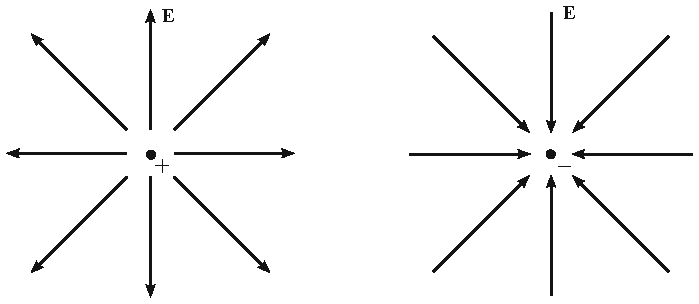
\includegraphics[width=0.829\linewidth]{images/vector/fig-12-1.pdf}
  \caption{带正电的粒子（左）与带负电的粒子（右）. 图中画出了从粒子发出的电场线. 电场线从正电荷向外指向、指向负电荷}
  \label{fig:12-1}
\end{figure}

假设我们有一个正电荷和一个负电荷，彼此相距一小段距离，如图~\ref{fig:12-2} 所示. 无论我们在哪里释放测试粒子，它都会同时感受到来自正电荷的排斥力和来自负电荷的吸引力. 排斥力与吸引力相对强弱取决于测试粒子到每个电荷的距离. 例如，在点 (a) 或 (c) 释放的测试粒子会感受到来自负电荷的一定吸引力和来自正电荷的一定排斥力. 在 (b) 处释放的测试粒子感受到的来自负电荷的吸引力远大于来自正电荷的排斥力. 而在 (d) 处释放的测试粒子感受到的来自正电荷的排斥力远大于来自负电荷的吸引力.

\begin{figure}[htbp]
  \centering
  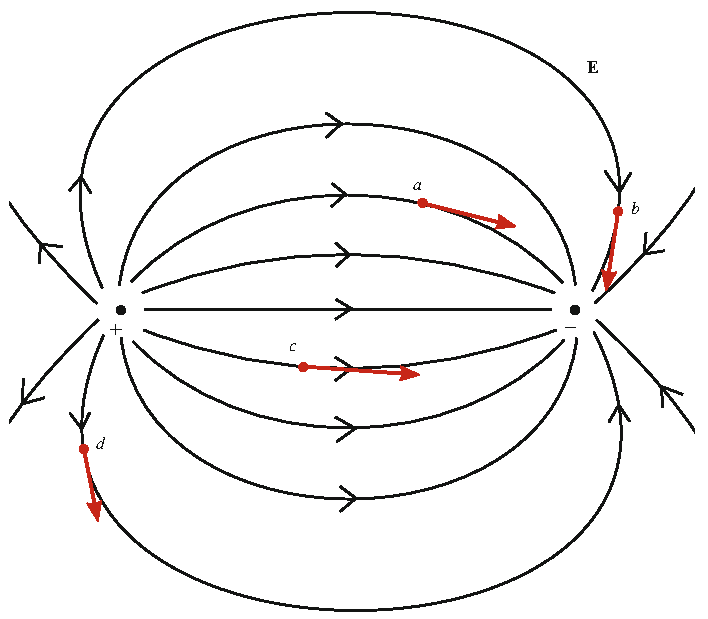
\includegraphics[width=0.840\linewidth]{images/vector/fig-12-2.pdf}
  \caption{相互靠近的一个带正电粒子与一个带负电粒子. 我们可以看到，一些从正电荷出发的电场线终止于负电荷}
  \label{fig:12-2}
\end{figure}

利用电场我们可以画出\newterm{electric-field-line}{电场线}{electric field line}. 电场线实际上是电场的积分曲线. 积分曲线是我们对向量场求积分时得到的路径，例如图~\ref{fig:2-19} 中显示了光滑向量场的积分曲线. 事实上，求向量场的积分曲线是流形上积分的一种途径，我们尚未讨论过它. 我们将在附录 B 中稍详细地讨论它. 在每个点，电场向量由电场线的切向量给出. 如果一个微小的正测试粒子在某个点被释放，它将沿着电场线运动，在每个点的速度由该点的电场向量给出. 一个点的向量长度告诉我们该点场的强弱. 在图像上，我们试图通过电场线画得有多密来显示空间某个区域中场有多强. 所以在图~\ref{fig:12-2} 中我们可以看到，离电荷越近，电场线越密，因而场越强；离电荷越远，电场线越疏，场越弱. 现在我们准备好陈述电场的高斯定律了. 这条定律涉及静电场.

\begin{center}
\fbox{\parbox{0.86\textwidth}{\centering
电场由电荷产生. 该电场穿过某个闭曲面的\newterm{flux}{通量}{flux}与闭曲面内部所包含的电荷量成正比.
}}
\end{center}

这条定律可以用向量微积分记号以两种不同方式表述：积分形式和微分形式. 正如其名称所示，积分形式涉及积分，微分形式涉及导数. 这两种形式是等价的. 首先我们给出电场的高斯定律的积分形式：
\[
\iint_S E\cdot\hat{n}\,dS=\frac{q_{\text{enc}}}{\varepsilon_0},
\]
其中
\begin{itemize}
  \item $E$ 是由电荷产生的静电场，
  \item $S$ 是闭曲面，
  \item $\hat{n}$ 是曲面 $S$ 的单位法向量，
  \item $dS$ 是曲面 $S$ 的面积元，
  \item $q_{\text{enc}}$ 是被曲面 $S$ 包围的电荷，以及
  \item $\varepsilon_0$ 是一个物理比例常数，称为\newterm{permittivity-of-free-space}{真空介电常数}{permittivity of free space}.
\end{itemize}
我们应该认识到 $\displaystyle\iint_S E\cdot\hat{n}\,dS$ 是场 $E$ 穿过曲面 $S$ 的通量. 由 $q_{\text{enc}}$ 产生、穿过闭曲面 $S$ 的 $E$ 的通量与 $q_{\text{enc}}$ 成正比，比例常数为 $\dfrac{1}{\varepsilon_0}$. 我们还需要认识到
\[
q_{\text{enc}}=\iiint_V\rho\,dV
\]
其中
\begin{itemize}
  \item $\rho$ 是\newterm{charge-density}{电荷密度}{charge density}，即 $\mathbb{R}^3$ 上描述每一点电荷量的一个函数.
\end{itemize}
我们在图~\ref{fig:12-3} 中展示了正在发生的事情. 一个闭曲面 $S$ 包围着若干个点电荷，有些是正的，有些是负的. 被包围的正电荷多于负电荷，所以当我们对 $S$ 上的电场向量场 $E$ 求积分时，得到离开曲面的正通量.

\begin{figure}[htbp]
  \centering
  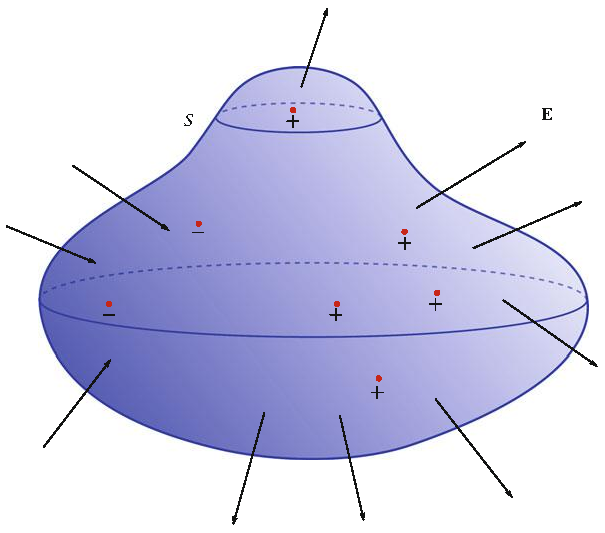
\includegraphics[width=0.717\linewidth]{images/vector/fig-12-3.pdf}
  \caption{包围若干正、负电荷的闭曲面 $S$. $S$ 内部的净电荷记为 $q_{\text{enc}}$. 图中画出了几条穿过 $S$ 的电场线. 由于正电荷多于负电荷，穿出 $S$ 的电场线多于穿入 $S$ 的电场线}
  \label{fig:12-3}
\end{figure}

利用向量微积分的散度定理，我们可以从电场的高斯定律的积分形式过渡到微分形式：
\[
\iint_{S=\partial V}E\cdot\hat{n}\,dS=\iiint_V\nabla\cdot E\,dV .
\]
注意我们用向量微积分记号 $\nabla\cdot E$ 表示 $\operatorname{div}E$. 把所有这些放在一起，我们得到
\begin{align*}
\iiint_V\nabla\cdot E\,dV&=\iint_S E\cdot\hat{n}\,dS && \text{散度定理}\\
&=\frac{q_{\text{enc}}}{\varepsilon_0} && \text{Gauss 定律}\\
&=\frac{1}{\varepsilon_0}\iiint_V\rho\,dV && \text{电荷密度的定义}\\
&=\iiint_V\frac{\rho}{\varepsilon_0}\,dV .
\end{align*}
令第一项与最后一项的被积函数相等，我们得到电场的高斯定律的微分形式：
\[
\nabla\cdot E=\frac{\rho}{\varepsilon_0}.
\]

\begin{question}\label{q:12-1}
把电场写成 $E=E_1\hat{\imath}+E_2\hat{\jmath}+E_3\hat{k}$，用 $E_1$、$E_2$、$E_3$ 写出电场的高斯定律. 做两次，一次针对电场的高斯定律的积分形式，一次针对其微分形式.
\end{question}

与电荷类似，磁性是亚原子粒子的一个内禀性质，尽管在许多方面它比电荷和电场要复杂一些. 我们可能合理地预期，正如电场由正负电荷产生，磁场由某种"磁荷"产生. 不幸的是，情况似乎并非如此. 这里我们将考虑旋转电子产生的磁场. 旋转质子和中子产生的场大约比电子产生的场小一千倍，因此常常可以忽略不计.

与电场 $E$ 一样，磁场用 $B$ 表示，存在于空间 $\mathbb{R}^3$ 中的每个点 $p$：
\[
B_p=\begin{bmatrix}B_1\\B_2\\B_3\end{bmatrix}_p .
\]
磁场可以用来给出\newterm{magnetic-field-line}{磁场线}{magnetic field line}，即磁场 $B$ 的积分曲线. 图~\ref{fig:12-4}、图~\ref{fig:12-5} 和图~\ref{fig:12-6} 中画出的正是这些磁场线，即 $B$ 的积分曲线，而不是 $B$ 本身. 与电场一样，唯一能知道磁场存在的方法是观察它如何与微小测试粒子相互作用. 和以前一样，我们考虑一个微小的带正电粒子. 然而，确定点 $p$ 处的磁场向量 $B_p$ 比求 $E_p$ 的情形要复杂一些. 我们不会深入细节，但这涉及观察一个运动的正测试粒子如何表现.

图~\ref{fig:12-4} 中显示了两个旋转的电子. 电子产生的磁场线取决于电子旋转的方向. 当然，我们把电子想象成实际上在旋转的一个微小球体，这本身就是帮助我们形象化电子是什么样、并思考这些物理性质如何表现的一幅卡通图. 像电子这样的亚原子粒子的真实量子力学本性，比这幅图让你相信的要复杂得多. 但就我们的目的而言，这幅图已经足够了.

\begin{figure}[htbp]
  \centering
  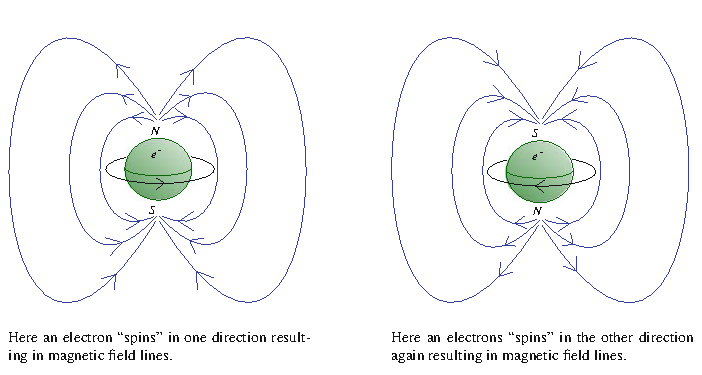
\includegraphics[width=0.851\linewidth]{images/vector/fig-12-4.pdf}
  \caption{把电子画成一个可以旋转的小球的卡通图. 磁场线的方向取决于电子的自旋，我们常常把自旋想象成球的旋转. 但要记住，电子真实的量子力学本性远比这幅图所描绘的复杂}
  \label{fig:12-4}
\end{figure}

产生磁场的较大的物体通常就称为\newterm{permanent-magnet}{永磁铁}{permanent magnet}，或者简单地称为磁铁. 人们一想到磁铁，往往会想到条形磁铁或图~\ref{fig:12-5} 中的马蹄形磁铁，或者图~\ref{fig:12-6} 中所示的冰箱贴. 构成这些磁铁的材料被磁化，从而产生自己持久的磁场. 这是因为材料的化学组成和晶体微观结构使亚原子粒子的磁场排列起来，从而产生更强的磁场.

\begin{figure}[htbp]
  \centering
  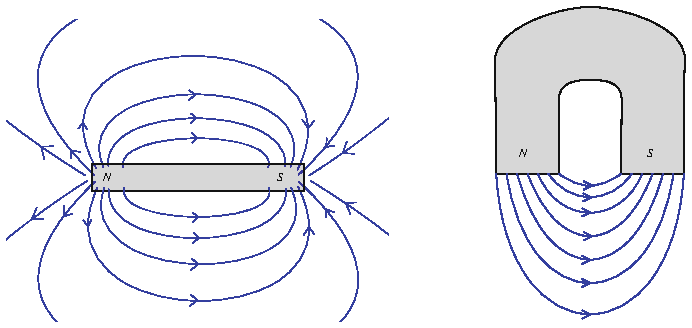
\includegraphics[width=0.960\linewidth]{images/vector/fig-12-5.pdf}
  \caption{条形磁铁（左）与马蹄形磁铁（右），图中标出了北极和南极. 磁感线以蓝色显示}
  \label{fig:12-5}
\end{figure}

\begin{figure}[htbp]
  \centering
  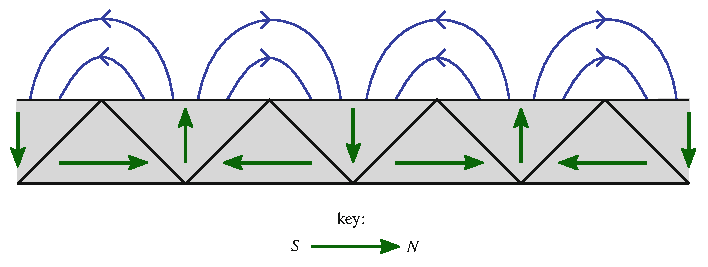
\includegraphics[width=0.840\linewidth]{images/vector/fig-12-6.pdf}
  \caption{冰箱贴的横截面. 注意磁南北方向发生变化的各个不同磁畴. 绿色箭头从南极指向北极. 磁场线以蓝色显示. 由于磁畴的性质，磁铁的一侧有磁场线，另一侧没有}
  \label{fig:12-6}
\end{figure}

在某些方面，磁场的高斯定律与电场的高斯定律非常相似，但其内容却非常不同. 这一差异之所以产生，是因为正电荷与负电荷可以彼此分开存在. 然而，磁北极却不可能与磁南极分开存在. 也就是说，北极和南极总是成对出现. 即使是一个旋转的电子也有北极和南极，如图~\ref{fig:12-4} 所示. \newterm{magnetic-monopole}{磁单极子}{magnetic monopole}，即孤立的北极或孤立的南极，从未在自然界中被观察到，也从未在实验室中被制造出来. 这意味着由一块同时具有北极和南极的磁铁产生的磁场会扭转回来、回到自身，正如我们从图~\ref{fig:12-4}、图~\ref{fig:12-5} 和图~\ref{fig:12-6} 中所看到的.

这种扭转的最终结果是，离开闭曲面的磁场总量也进入同一个闭曲面，因此穿过该闭曲面的净磁通量总是为零. 这就引出了磁场的高斯定律.

\begin{center}
\fbox{\parbox{0.86\textwidth}{\centering
磁场由磁铁产生. 该磁场穿过某个闭曲面的通量为零.
}}
\end{center}

同样，这条定律也可以用向量微积分记号以两种不同方式表述：积分形式和微分形式. 积分形式为
\[
\iint_S B\cdot\hat{n}\,dS=0,
\]
其中
\begin{itemize}
  \item $B$ 是磁场，
  \item $S$ 是闭曲面，
  \item $\hat{n}$ 是曲面 $S$ 的单位法向量，以及
  \item $dS$ 是曲面 $S$ 的面积元.
\end{itemize}
考虑图~\ref{fig:12-7}，我们可以看到磁场的高斯定律的含义. 图中画出的是一块磁铁的二维截面，连同代表向量场 $B$ 的磁场线. 蓝色的闭曲线代表闭曲面. 从图中可以看出，每条进入闭曲面的磁场线也离开该闭曲面.

\begin{figure}[htbp]
  \centering
  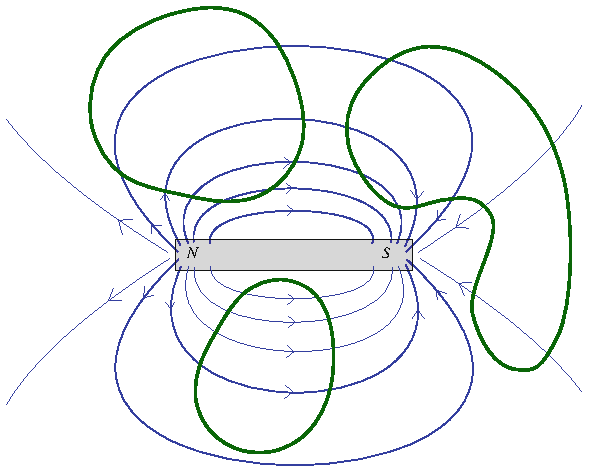
\includegraphics[width=0.698\linewidth]{images/vector/fig-12-7.pdf}
  \caption{图中显示一块具有北极和南极的磁铁，以及"折返"回到自身的磁场线. 从绿色的"闭曲面"可以看出，进入曲面的磁场线条数恰好等于离开曲面的条数，因此穿过任何曲面的磁通量总是为零}
  \label{fig:12-7}
\end{figure}

用散度定理导出磁场的高斯定律的微分形式就是轻而易举的了：
\begin{align*}
\iiint_V\nabla\cdot B\,dV&=\iint_S B\cdot\hat{n}\,dS && \text{散度定理}\\
&=0 && \text{Gauss 定律}\\
&=\iiint_V 0\,dV .
\end{align*}
令第一项与最后一项的被积函数相等，我们得到磁场的高斯定律的微分形式：
\[
\nabla\cdot B=0.
\]

\begin{question}\label{q:12-2}
把磁场写成 $B=B_1\hat{\imath}+B_2\hat{\jmath}+B_3\hat{k}$，用 $B_1$、$B_2$、$B_3$ 写出磁场的高斯定律. 做两次，一次针对磁场的高斯定律的积分形式，一次针对其微分形式.
\end{question}

\section{Faraday 定律与 Ampère-Maxwell 定律}

Faraday 定律和 Ampère-Maxwell 定律都解释了电场与磁场之间的关系. 我们先来看 Faraday 定律. Faraday 定律中的感应电场 $E$ 与电场的高斯定律中的静电场 $E$ 类似，但结构不同. 两种场都作为力来加速带电粒子，但静电场的场线始于正电荷、止于负电荷，而感应电场的场线则环回自身. Faraday 定律的陈述非常简单.

\begin{center}
\fbox{\parbox{0.86\textwidth}{\centering
穿过曲面的变化磁通量在该曲面边界周围感应出一个环流的电场.
}}
\end{center}

换言之，穿过曲面 $S$ 的变化磁通量产生一个绕着 $S$ 的边界、即绕着 $C=\partial S$ 环流的电场. 考虑图~\ref{fig:12-8}. 当磁铁移动时，穿过假想的浅绿色曲面的磁通量沿该曲面的边界感应出一个电场. 感应电场环绕的方向取决于穿过假想曲面的磁通量是在增大还是在减小. 这里的关键是，穿过曲面的磁通量必须随时间变化. 如果穿过曲面的磁通量不随时间变化，就不会感应出电场.

\begin{figure}[htbp]
  \centering
  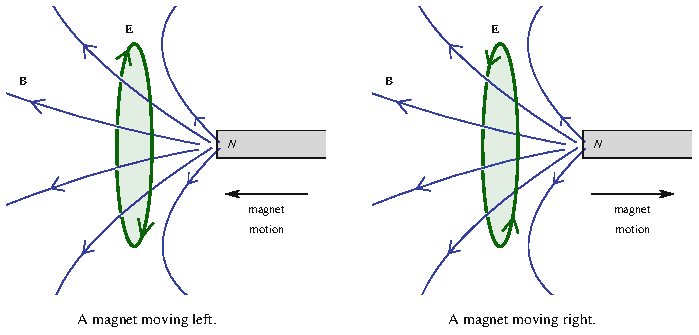
\includegraphics[width=0.960\linewidth]{images/vector/fig-12-8.pdf}
  \caption{变化的磁场在曲面边界周围产生环流的电场. 感应电场的环绕方向取决于磁通量是在增大还是在减小}
  \label{fig:12-8}
\end{figure}

Faraday 定律的积分形式为
\[
\oint_C E\cdot\hat{t}\,ds=-\frac{d}{dt}\iint_S B\cdot\hat{n}\,dS .
\]
Faraday 定律的另一种写法是
\[
\oint_C E\cdot\hat{t}\,ds=-\iint_S\frac{\partial B}{\partial t}\cdot\hat{n}\,dS .
\]
我们不会讨论这里交换导数与积分次序何以是允许的，这我们留给分析课程. 在 Faraday 定律的这两个版本中都有
\begin{itemize}
  \item $E$ 是沿曲线 $C$ 的感应电场，
  \item $C=\partial S$ 是闭曲线，即曲面 $S$ 的边界，
  \item $ds$ 是 $C$ 的线元，
  \item $\hat{t}$ 是 $C$ 的单位切向量，
  \item $B$ 是磁场，
  \item $\hat{n}$ 是曲面 $S$ 的单位法向量，以及
  \item $dS$ 是 $S$ 的面积元.
\end{itemize}
为了从 Faraday 定律的积分形式过渡到微分形式，我们将使用向量微积分版本的 Stokes 定理：
\[
\iint_S(\nabla\times E)\cdot\hat{n}\,dS=\oint_{\partial S=C}E\cdot\hat{t}\,ds .
\]
把所有这些放在一起，我们有
\begin{align*}
\iint_S(\nabla\times E)\cdot\hat{n}\,dS&=\oint_{\partial S=C}E\cdot\hat{t}\,ds && \text{Stokes 定理}\\
&=-\iint_S\frac{\partial B}{\partial t}\cdot\hat{n}\,dS && \text{Faraday 定律} .
\end{align*}
令第一项与最后一项的被积函数相等，我们得到 Faraday 定律的微分形式
\[
\nabla\times E=-\frac{\partial B}{\partial t}.
\]

\begin{question}\label{q:12-3}
设 $E=E_1\hat{\imath}+E_2\hat{\jmath}+E_3\hat{k}$，$B=B_1\hat{\imath}+B_2\hat{\jmath}+B_3\hat{k}$，用 $E_1$、$E_2$、$E_3$ 和 $B_1$、$B_2$、$B_3$ 写出 Faraday 定律. 你将得到三个独立的方程. 做两次，一次针对 Faraday 定律的积分形式，一次针对其微分形式.
\end{question}

现在我们把注意力转向 Ampère-Maxwell 定律. 这条定律与其他定律略有不同，因为它的右边有两项，一项涉及电流，另一项涉及电通量. Ampère-Maxwell 定律陈述如下：

\begin{center}
\fbox{\parbox{0.86\textwidth}{\centering
穿过曲面的电流或变化的电通量在曲面边界周围产生环流的磁场.
}}
\end{center}

与之前的定律不同，这条定律的右边有两项. 第一项涉及电流如何感应出磁场. 假设我们有一根导线，电流 $I$ 沿着它流动. 电流就是流动的电子. 如果有一个曲面 $S$，边界为 $C=\partial S$，而载流导线穿过或穿透该曲面，那么电流就沿曲面边界感应出磁场. 如果导线不穿过该曲面，那么边界周围就没有感应磁场. 见图~\ref{fig:12-9}. 当然，这对导线穿过的任何曲面都成立. 考虑图~\ref{fig:12-10}. 磁场沿着导线的整个长度被感应出来.

\begin{figure}[htbp]
  \centering
  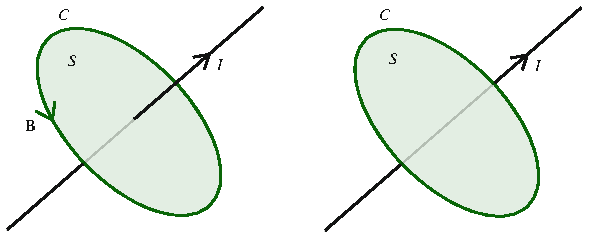
\includegraphics[width=0.698\linewidth]{images/vector/fig-12-9.pdf}
  \caption{沿导线流动的电流 $I$. 左图中载流导线"穿透"绿色曲面 $S$，从而在曲面边界 $C=\partial S$ 周围产生环流磁场. 由于电流穿过曲面，我们记为 $I_{\text{enc}}$. 右图中载流导线不穿过曲面，因此边界周围没有磁场}
  \label{fig:12-9}
\end{figure}

\begin{figure}[htbp]
  \centering
  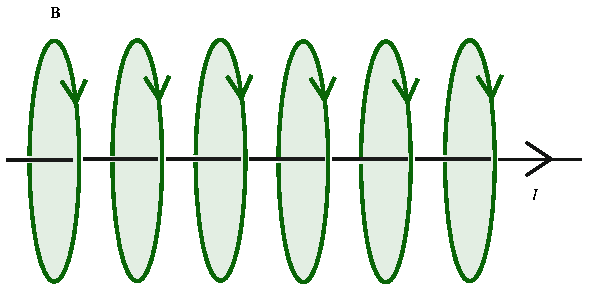
\includegraphics[width=0.698\linewidth]{images/vector/fig-12-10.pdf}
  \caption{与图~\ref{fig:12-9} 类似，沿导线流动的电流在导线周围感应出磁场. 当然，磁场并不限于某一个曲面的边界，它出现在导线所穿过的每一个曲面的边界上}
  \label{fig:12-10}
\end{figure}

第二项涉及变化的电场. 在图~\ref{fig:12-11} 中我们显示了三个电荷，两个负的和一个正的，连同曲面 $S$ 及其边界 $C=\partial S$. 这三个电荷产生一个电场. 图中画出了几条电场线，正如我们所看到的，其中一些电场线穿过该曲面. 当这三个电荷运动时（如附在电荷上的速度箭头所示），运动电荷感应出的电场随时间变化. 这意味着穿过曲面的电通量也在变化，从而在曲面边界周围感应出磁场.

\begin{figure}[htbp]
  \centering
  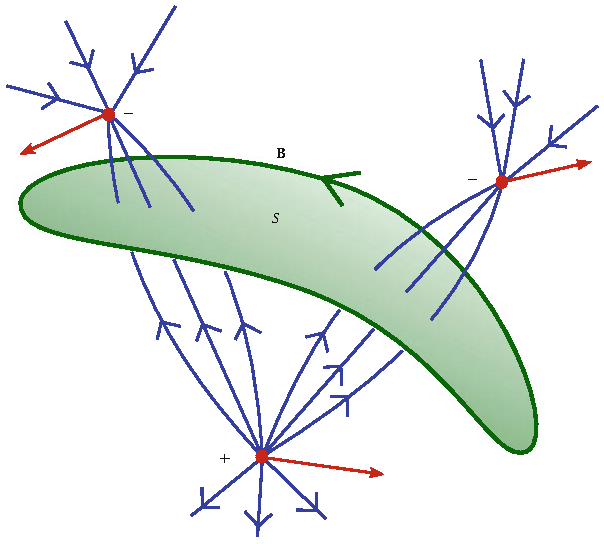
\includegraphics[width=0.756\linewidth]{images/vector/fig-12-11.pdf}
  \caption{这里三个电荷（红色）感应出一个电场. 图中画出了几条电场线（蓝色），它们穿过曲面 $S$（绿色）. 如果电荷在运动，如从电荷发出的速度矢量（红色）所示，那么电场随时间变化，从而沿曲面边界 $\partial S$ 感应出磁场}
  \label{fig:12-11}
\end{figure}

Ampère-Maxwell 定律把感应磁场的这两种不同方式结合起来. 图~\ref{fig:12-12} 试图同时展示这两种情形. 电荷在运动，从而使电场变化，同时电流在导线中流动. 沿曲面边界的磁场是这两者各自产生的场之和. 现在我们准备好陈述 Ampère-Maxwell 定律的数学形式了. 它的积分形式为
\[
\oint_C B\cdot\hat{t}\,ds=\mu_0 I_{\text{enc}}+\mu_0\varepsilon_0\frac{d}{dt}\iint_S E\cdot\hat{n}\,dS .
\]
Ampère-Maxwell 定律的另一种写法是
\[
\oint_C B\cdot\hat{t}\,ds=\mu_0 I_{\text{enc}}+\mu_0\varepsilon_0\iint_S\frac{\partial E}{\partial t}\cdot\hat{n}\,dS .
\]

\begin{figure}[htbp]
  \centering
  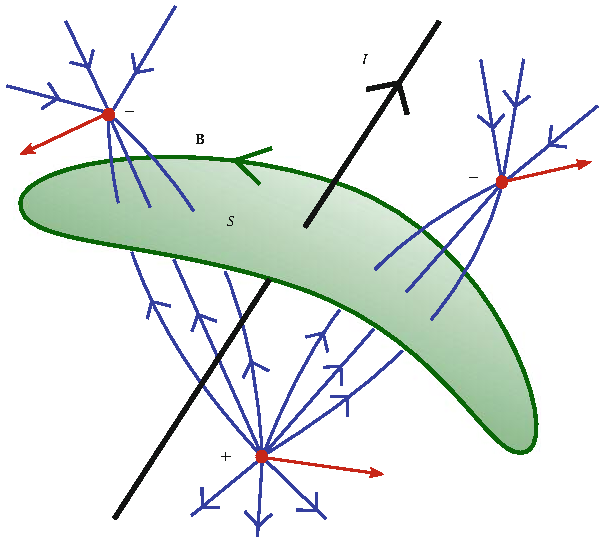
\includegraphics[width=0.756\linewidth]{images/vector/fig-12-12.pdf}
  \caption{这里，如图~\ref{fig:12-9} 左图所示的沿导线电流与如图~\ref{fig:12-11} 所示的变化电场这两种效应结合起来，产生沿 $\partial S$ 的磁场}
  \label{fig:12-12}
\end{figure}

同样，我们不会讨论这里交换导数与积分次序何以是允许的. 在这两个版本中都有
\begin{itemize}
  \item $\mu_0$ 是空间的磁导率，以及
  \item $I_{\text{enc}}$ 是被包围的电流.
\end{itemize}
由于电流不过是流动的电子，我们有电流 $I$ 是流动电荷密度 $J=J_1\hat{\imath}+J_2\hat{\jmath}+J_3\hat{k}$ 的积分：
\[
I=\iint_S J\cdot\hat{n}\,dS .
\]
再次利用向量微积分版本的 Stokes 定理，我们有
\begin{align*}
\iint_S(\nabla\times B)\cdot\hat{n}\,dS&=\oint_C B\cdot\hat{t}\,ds && \text{Stokes 定理}\\
&=\mu_0 I_{\text{enc}}+\mu_0\varepsilon_0\iint_S\frac{\partial E}{\partial t}\cdot\hat{n}\,dS && \text{Ampère-Maxwell 定律}\\
&=\mu_0\iint_S J\cdot\hat{n}\,dS+\mu_0\varepsilon_0\iint_S\frac{\partial E}{\partial t}\cdot\hat{n}\,dS && \text{电流密度的定义}\\
&=\iint_S\mu_0 J\cdot\hat{n}\,dS+\iint_S\mu_0\varepsilon_0\frac{\partial E}{\partial t}\cdot\hat{n}\,dS\\
&=\iint_S\left(\mu_0 J+\mu_0\varepsilon_0\frac{\partial E}{\partial t}\right)\cdot\hat{n}\,dS .
\end{align*}
倒数第二个等式只是记号上的改变. 令第一项与最后一项的被积函数相等，我们得到 Ampère-Maxwell 定律的微分形式：
\[
\nabla\times B=\mu_0 J+\mu_0\varepsilon_0\frac{\partial E}{\partial t}.
\]

\begin{question}\label{q:12-4}
设 $E=E_1\hat{\imath}+E_2\hat{\jmath}+E_3\hat{k}$，$B=B_1\hat{\imath}+B_2\hat{\jmath}+B_3\hat{k}$，$J=J_1\hat{\imath}+J_2\hat{\jmath}+J_3\hat{k}$，用 $E_1$、$E_2$、$E_3$、$B_1$、$B_2$、$B_3$ 和 $J_1$、$J_2$、$J_3$ 写出 Ampère-Maxwell 定律. 你将得到三个独立的方程. 做两次，一次针对 Ampère-Maxwell 定律的积分形式，一次针对其微分形式.
\end{question}

此后我们将轻率地假设单位已经选取得使得 $\mu_0=\varepsilon_0=1$. 这省去了我们到处携带一大堆常数的麻烦，却让物理学家和工程师抓狂. 这就给出如下 Maxwell 方程组的总结：

\begin{center}
\fbox{\parbox{0.95\textwidth}{\centering
\textbf{Maxwell 方程组：版本一}\\[2pt]
\begin{tabular}{@{}c@{\quad}c@{}}
\textbf{积分形式} & \textbf{微分形式}\\[2pt]
$\displaystyle\iint_S E\cdot\hat{n}\,dS=q_{\text{enc}}$ & $\nabla\cdot E=\rho$\\[2pt]
$\displaystyle\iint_S B\cdot\hat{n}\,dS=0$ & $\nabla\cdot B=0$\\[2pt]
$\displaystyle\oint_C E\cdot\hat{t}\,ds=-\iint_S\frac{\partial B}{\partial t}\cdot\hat{n}\,dS$ & $\nabla\times E=-\dfrac{\partial B}{\partial t}$\\[2pt]
$\displaystyle\oint_C B\cdot\hat{t}\,ds=I_{\text{enc}}+\iint_S\frac{\partial E}{\partial t}\cdot\hat{n}\,dS$ & $\nabla\times B=J+\dfrac{\partial E}{\partial t}$
\end{tabular}
}}
\end{center}

\section{狭义相对论与 Hodge 对偶}

现在我们想用微分形式来重新表述电磁学. 实际上有几种方法可以做到这一点. 首先，可以在三维欧几里得空间上使用形式，并把时间作为一个单独的变量. 然而，这种方法最终不够优雅. 事实上，这种方法未能发挥微分形式的全部威力，也未能阐明电磁学最有趣的特征之一，即它与狭义相对论相容. 有趣的是，在十九世纪物理学的两大领域——经典力学与经典电磁学——中，与狭义相对论相容的是经典电磁学，而不是经典力学.

换言之，Maxwell 方程组在高速下不需要任何修改，这并不奇怪，因为它们与以光速传播的电磁场有关. 然而，经典力学在接近光速的速度下是极其不准确的. Maxwell 的电磁理论已经是完全相对论性的，当我们从向量微积分表述转向该理论的微分形式表述时，这一事实可以清楚地看到.

然而，在转向 Maxwell 方程组的微分形式表述之前，我们需要做一些修改. 首先，我们需要转到四维. 但我们将不考虑标准的欧几里得空间 $\mathbb{R}^4$，而考虑闵可夫斯基空间，即狭义相对论所建立的四维流形. 闵可夫斯基流形有时记为 $M^4$ 或 $\mathbb{R}^{1,3}$，其中时间变量与三个空间变量分开. 我们将使用记号 $\mathbb{R}^{1,3}$.

闵可夫斯基空间 $\mathbb{R}^{1,3}$ 与欧几里得空间 $\mathbb{R}^4$ 不同，因为它的度量张量不同. 度量在第 10.1 节非正式地讨论过，并将在 A.6 节正式定义和讨论. 闵可夫斯基空间这种不同的度量张量意味着 $\mathbb{R}^{1,3}$ 具有与 $\mathbb{R}^4$ 不同的内积，即点积. 我们首先考虑 $\mathbb{R}^4$ 上关于标准基的欧几里得度量. 这个欧几里得度量可以用矩阵
\[
\begin{bmatrix}
1&0&0&0\\
0&1&0&0\\
0&0&1&0\\
0&0&0&1
\end{bmatrix}
\]
表示. 内积，即点积，可以用这个矩阵计算. 这是我们在第 5.6 节看到过的东西. 设 $v$ 和 $w$ 是 $\mathbb{R}^4$ 中某点 $p\in\mathbb{R}^4$ 处的两个向量. 也就是说，$v,w\in T_p\mathbb{R}^4$. 如果 $\mathbb{R}^4$ 的标准基记为 $e_1,e_2,e_3,e_4$，那么在 Einstein 求和记号下，我们有 $v=v^ie_i$，$w=w^ie_i$，$1\leq i\leq4$. 于是内积由
\[
\begin{aligned}
v\cdot w\equiv\langle v,w\rangle
&=v^T\begin{bmatrix}1&0&0&0\\0&1&0&0\\0&0&1&0\\0&0&0&1\end{bmatrix}w\\
&=[v^1,v^2,v^3,v^4]\begin{bmatrix}1&0&0&0\\0&1&0&0\\0&0&1&0\\0&0&0&1\end{bmatrix}\begin{bmatrix}w^1\\w^2\\w^3\\w^4\end{bmatrix}\\
&=v^1w^1+v^2w^2+v^3w^3+v^4w^4 .
\end{aligned}
\]
闵可夫斯基空间 $\mathbb{R}^{1,3}$ 上的度量称为\newterm{minkowski-metric}{闵可夫斯基度量}{Minkowski metric}，它的定义略有不同. 我们首先把 $\mathbb{R}^{1,3}$ 的标准基记为 $e_0,e_1,e_2,e_3$，其中 $e_0$ 是时间方向的单位向量，$e_1$ 是 $x$ 方向的单位向量，$e_2$ 是 $y$ 方向的单位向量，$e_3$ 是 $z$ 方向的单位向量. $\mathbb{R}^{1,3}$ 上关于这个基的度量用矩阵
\[
\begin{bmatrix}
-1&0&0&0\\
0&1&0&0\\
0&0&1&0\\
0&0&0&1
\end{bmatrix}
\]
表示. 这里我们应该注意，有些书使用矩阵
\[
\begin{bmatrix}
1&0&0&0\\
0&-1&0&0\\
0&0&-1&0\\
0&0&0&-1
\end{bmatrix}
\]
来代替. 这只会导致所有符号被颠倒. 究竟使用这个矩阵的哪个版本，实际上是一个品味和约定的问题，尽管第一个似乎用得稍多一些. 但你应该仔细检查你所读的书中使用的是哪个约定.

设 $v$ 和 $w$ 是 $\mathbb{R}^{1,3}$ 中某点 $p\in\mathbb{R}^{1,3}$ 处的两个向量，即 $v,w\in T_p\mathbb{R}^{1,3}$. 那么在 Einstein 求和记号下，我们有 $v=v^ie_i$，$w=w^ie_i$，$0\leq i\leq3$. 内积可以由
\[
\begin{aligned}
\langle v,w\rangle
&=v^T\begin{bmatrix}-1&0&0&0\\0&1&0&0\\0&0&1&0\\0&0&0&1\end{bmatrix}w\\
&=[v^0,v^1,v^2,v^3]\begin{bmatrix}-1&0&0&0\\0&1&0&0\\0&0&1&0\\0&0&0&1\end{bmatrix}\begin{bmatrix}w^0\\w^1\\w^2\\w^3\end{bmatrix}\\
&=-v^0w^0+v^1w^1+v^2w^2+v^3w^3 .
\end{aligned}
\]
注意我们没有在这里使用点积记号. 点积 $v\cdot w$ 一般保留用于使用欧几里得度量的情形，而括号记号 $\langle v,w\rangle$ 常常与其他度量一起使用. 另外，如果你还记得，我们用括号记号表示 1-形式与向量之间的配对，$\langle\alpha,v\rangle\equiv\alpha(v)$，偶尔你也会看到它用于 $k$-形式，$\langle\alpha,(v_1,\ldots,v_k)\rangle\equiv\alpha(v_1,\ldots,v_k)$. 很容易判断 $\langle\cdot,\cdot\rangle$ 是在何种意义上被使用的，只需看看里面是什么：两个向量，还是一个形式与一个向量或一组向量.

现在我们还需要做一些定义，并整理好记号. 首先，我们用 $x^1$ 表示 $x$，用 $x^2$ 表示 $y$，用 $x^3$ 表示 $z$. $t$ 要么保持不变，要么记为 $x^0$. 目前我们继续用 $t$ 而不用 $x^0$，以帮助你记住它是时间变量. 我们在闵可夫斯基空间 $\mathbb{R}^{1,3}$ 的每一点定义如下向量空间：
\begin{align*}
f,g\in\bigwedge_p^0(\mathbb{R}^{1,3})=\{\mathbb{R}^{1,3}\text{ 上的连续函数}\}, \\
\alpha,\beta\in\bigwedge_p^1(\mathbb{R}^{1,3})=T_p^*\mathbb{R}^{1,3}=\operatorname{span}\{dt,dx^1,dx^2,dx^3\}, \\
\gamma,\delta\in\bigwedge_p^2(\mathbb{R}^{1,3})=\operatorname{span}\{dt\wedge dx^1,\,dt\wedge dx^2,\,dt\wedge dx^3,\,dx^1\wedge dx^2,\,dx^2\wedge dx^3,\,dx^3\wedge dx^1\}, \\
\omega,\nu\in\bigwedge_p^3(\mathbb{R}^{1,3})=\operatorname{span}\{dt\wedge dx^1\wedge dx^2,\,dt\wedge dx^3\wedge dx^1,\,dt\wedge dx^2\wedge dx^3,\,dx^1\wedge dx^2\wedge dx^3\}, \\
\varepsilon,\theta\in\bigwedge_p^4(\mathbb{R}^{1,3})=\operatorname{span}\{dt\wedge dx^1\wedge dx^2\wedge dx^3\}.
\end{align*}
作为惯例，在书写各个空间的基元素时，我们先写 $dt$，其余各项按循环次序排列. 我们将
\begin{align*}
\alpha & =\alpha_0\,dt+\alpha_1\,dx^1+\alpha_2\,dx^2+\alpha_3\,dx^3, \\
\gamma & =\gamma_{01}\,dt\wedge dx^1+\gamma_{02}\,dt\wedge dx^2+\gamma_{03}\,dt\wedge dx^3
+\gamma_{12}\,dx^1\wedge dx^2 \\
& \quad +\gamma_{23}\,dx^2\wedge dx^3+\gamma_{31}\,dx^3\wedge dx^1, \\
\omega & =\omega_{012}\,dt\wedge dx^1\wedge dx^2+\omega_{031}\,dt\wedge dx^3\wedge dx^1+\omega_{023}\,dt\wedge dx^2\wedge dx^3+\omega_{123}\,dx^1\wedge dx^2\wedge dx^3, \\
\varepsilon & =\varepsilon_{0123}\,dt\wedge dx^1\wedge dx^2\wedge dx^3,
\end{align*}
而 $\beta$、$\delta$、$\nu$、$\theta$ 的写法类似. 用来跟踪系数的下标与基元素相对应.

我们取所有 $\bigwedge_p^0(\mathbb{R}^{1,3})$（$p\in\mathbb{R}^{1,3}$）的不交并，得到空间 $\bigwedge^0(\mathbb{R}^{1,3})$，从而把 $\bigwedge^0(\mathbb{R}^{1,3})$ 做成流形 $\mathbb{R}^{1,3}$ 上的一个丛. 空间 $\bigwedge^1(\mathbb{R}^{1,3})$、$\bigwedge^2(\mathbb{R}^{1,3})$、$\bigwedge^3(\mathbb{R}^{1,3})$ 和 $\bigwedge^4(\mathbb{R}^{1,3})$ 也类似地得到. 然后我们可以在这些空间上定义内积.

由于这些空间中有些的基元素很多，我们把写出这些向量空间的度量矩阵留作练习. 然而，所有内积本质上都是沿底层流形 $\mathbb{R}^{1,3}$ 使用闵可夫斯基度量定义内积时的同样思路定义的；任何含有 $dt$ 的项都有一个负号. 于是我们有
\begin{align*}
f,g\in\bigwedge^0(\mathbb{R}^{1,3});\quad \langle f,g\rangle=f\cdot g, \\
\alpha,\beta\in\bigwedge^1(\mathbb{R}^{1,3});\quad \langle\alpha,\beta\rangle=-\alpha_0\beta_0+\alpha_1\beta_1+\alpha_2\beta_2+\alpha_3\beta_3, \\
\gamma,\delta\in\bigwedge^2(\mathbb{R}^{1,3});\quad \langle\gamma,\delta\rangle=-\gamma_{01}\delta_{01}-\gamma_{02}\delta_{02}-\gamma_{03}\delta_{03}+\gamma_{12}\delta_{12}+\gamma_{23}\delta_{23}+\gamma_{31}\delta_{31}, \\
\omega,\nu\in\bigwedge^3(\mathbb{R}^{1,3});\quad \langle\omega,\nu\rangle=-\omega_{012}\nu_{012}-\omega_{023}\nu_{023}-\omega_{031}\nu_{031}+\omega_{123}\nu_{123}, \\
\varepsilon,\theta\in\bigwedge^4(\mathbb{R}^{1,3});\quad \langle\varepsilon,\theta\rangle=-\varepsilon_{0123}\theta_{0123}.
\end{align*}
内积是逐点定义的，例如在点 $p$ 处有 $\langle f,g\rangle_p=f(p)g(p)$，$\langle\alpha,\beta\rangle_p=-\alpha_0(p)\beta_0(p)+\alpha_1(p)\beta_1(p)+\alpha_2(p)\beta_2(p)+\alpha_3(p)\beta_3(p)$，等等. 因此，如果用来定义形式的函数都是流形 $\mathbb{R}^{1,3}$ 上的光滑函数，那么两个 $k$-形式（$k=0,1,2,3,4$）的内积就是 $\mathbb{R}^{1,3}$ 上的光滑函数. 例如，我们有 $\langle f,g\rangle:\mathbb{R}^{1,3}\to\mathbb{R}$，等等.

\begin{question}\label{q:12-5}
写出空间 $\bigwedge^0(\mathbb{R}^{1,3})$、$\bigwedge^1(\mathbb{R}^{1,3})$、$\bigwedge^2(\mathbb{R}^{1,3})$、$\bigwedge^3(\mathbb{R}^{1,3})$ 和 $\bigwedge^4(\mathbb{R}^{1,3})$ 的度量矩阵.
\end{question}

我们需要利用这些新的内积求出 Hodge 星算子. 在 $\mathbb{R}^{1,3}$ 上，微分形式 $\beta$ 的 Hodge 星对偶由公式
\[
\alpha\wedge\ast\beta=\langle\alpha,\beta\rangle\,dt\wedge dx^1\wedge dx^2\wedge dx^3
\]
给出. 如果 $\alpha$ 是一个基元素，那么求 $\ast\alpha$ 的公式简化为
\[
\alpha\wedge\ast\alpha=\langle\alpha,\alpha\rangle\,dt\wedge dx^1\wedge dx^2\wedge dx^3=\pm\,dt\wedge dx^1\wedge dx^2\wedge dx^3
\]
其中负号还是正号取决于元素 $\alpha$ 是否含有 $dt$.

现在我们求 1-形式基元素的 Hodge 星对偶. 注意我们总是先写 $dt$，其余所有元素按循环次序排列：
\begin{align*}
\begin{aligned}
dt\wedge\ast dt&=\langle dt,dt\rangle\,dt\wedge dx^1\wedge dx^2\wedge dx^3\\
&=-dt\wedge dx^1\wedge dx^2\wedge dx^3\\
&\Rightarrow\ast dt=-dx^1\wedge dx^2\wedge dx^3,
\end{aligned} \\
\begin{aligned}
dx^1\wedge\ast dx^1&=\langle dx^1,dx^1\rangle\,dt\wedge dx^1\wedge dx^2\wedge dx^3\\
&=dt\wedge dx^1\wedge dx^2\wedge dx^3\\
&=-dx^1\wedge dt\wedge dx^2\wedge dx^3\\
&\Rightarrow\ast dx^1=-dt\wedge dx^2\wedge dx^3,
\end{aligned}
\end{align*}
其余两个基元素的计算类似. 于是 1-形式基元素的 Hodge 对偶为
\begin{align*}
\ast dt=-dx^1\wedge dx^2\wedge dx^3, \\
\ast dx^1=-dt\wedge dx^2\wedge dx^3, \\
\ast dx^2=-dt\wedge dx^3\wedge dx^1, \\
\ast dx^3=-dt\wedge dx^1\wedge dx^2 .
\end{align*}

\begin{question}\label{q:12-6}
做计算求出 $dx^2$ 和 $dx^3$ 的 Hodge 星对偶.
\end{question}

2-形式基元素的 Hodge 对偶同样求出. 同样，我们总是先写 $dt$，并在需要时把其余元素按循环次序排列：
\begin{align*}
\begin{aligned}
(dt\wedge dx^1)\wedge\ast(dt\wedge dx^1)&=\langle dt\wedge dx^1,dt\wedge dx^1\rangle\,dt\wedge dx^1\wedge dx^2\wedge dx^3\\
&=-(dt\wedge dx^1)\wedge(dx^2\wedge dx^3)\\
&\Rightarrow\ast(dt\wedge dx^1)=-dx^2\wedge dx^3,
\end{aligned} \\
\begin{aligned}
(dt\wedge dx^2)\wedge\ast(dt\wedge dx^2)&=\langle dt\wedge dx^2,dt\wedge dx^2\rangle\,dt\wedge dx^1\wedge dx^2\wedge dx^3\\
&=-dt\wedge dx^2\wedge dx^3\wedge dx^1\\
&\Rightarrow\ast(dt\wedge dx^2)=-dx^3\wedge dx^1 .
\end{aligned}
\end{align*}
其余基元素的计算类似. 总结起来，2-形式基元素的 Hodge 对偶为
\begin{align*}
\ast(dt\wedge dx^1)=-dx^2\wedge dx^3, \\
\ast(dt\wedge dx^2)=-dx^3\wedge dx^1, \\
\ast(dt\wedge dx^3)=-dx^1\wedge dx^2, \\
\ast(dx^1\wedge dx^2)=dt\wedge dx^3, \\
\ast(dx^2\wedge dx^3)=dt\wedge dx^1, \\
\ast(dx^3\wedge dx^1)=dt\wedge dx^2 .
\end{align*}

\begin{question}\label{q:12-7}
做计算求出其余 2-形式基元素的 Hodge 星对偶.
\end{question}

\begin{question}\label{q:12-8}
求 $\alpha=7\,dt\wedge dx^2-20\,dt\wedge dx^3+6\,dx^2\wedge dx^3-2\,dx^3\wedge dx^1$ 的 $\ast\alpha$.
\end{question}

最后，3-形式基元素的 Hodge 星对偶为
\begin{align*}
\ast(dt\wedge dx^1\wedge dx^2)=-dx^3, \\
\ast(dt\wedge dx^2\wedge dx^3)=-dx^1, \\
\ast(dt\wedge dx^3\wedge dx^1)=-dx^2, \\
\ast(dx^1\wedge dx^2\wedge dx^3)=-dt .
\end{align*}

\begin{question}\label{q:12-9}
做计算求出 3-形式基元素的 Hodge 星对偶.
\end{question}

\section{微分形式表述}

既然我们已具备必要的数学基础，就可以着手实现本章的主要目的：用微分形式写出 Maxwell 方程组. 回想一下，在向量微积分记号中，电场和磁场写作
\begin{align*}
E=E_1\hat{\imath}+E_2\hat{\jmath}+E_3\hat{k}, \\
B=B_1\hat{\imath}+B_2\hat{\jmath}+B_3\hat{k}.
\end{align*}
我们将把这两个场组合起来，构成 $\mathbb{R}^{1,3}$ 上一种特殊的 2-形式，称为\newterm{faraday-two-form}{Faraday 2-形式}{Faraday two-form}. 尽管形式一般用希腊字母表示，但由于历史原因，这个特殊形式用 $F$ 表示. 另外，这个 2-形式的系数下标并不遵循 2-形式的下标约定，而是保留 $E$ 和 $B$ 原来的下标. Faraday 2-形式为

\begin{center}
\fbox{\parbox{0.95\textwidth}{\centering
\textbf{Faraday 2-形式}\\[2pt]
$F=-E_1\,dt\wedge dx^1-E_2\,dt\wedge dx^2-E_3\,dt\wedge dx^3+B_1\,dx^2\wedge dx^3+B_2\,dx^3\wedge dx^1+B_3\,dx^1\wedge dx^2$
}}
\end{center}

现在我们费力地完成 $dF$ 的计算：
\[
\begin{aligned}
dF={}&-dE_1\wedge dt\wedge dx^1-dE_2\wedge dt\wedge dx^2-dE_3\wedge dt\wedge dx^3\\
&+dB_1\wedge dx^2\wedge dx^3+dB_2\wedge dx^3\wedge dx^1+dB_3\wedge dx^1\wedge dx^2\\
={}&-\left(\frac{\partial E_1}{\partial t}\,dt+\frac{\partial E_1}{\partial x^1}\,dx^1+\frac{\partial E_1}{\partial x^2}\,dx^2+\frac{\partial E_1}{\partial x^3}\,dx^3\right)\wedge dt\wedge dx^1\\
&-\left(\frac{\partial E_2}{\partial t}\,dt+\frac{\partial E_2}{\partial x^1}\,dx^1+\frac{\partial E_2}{\partial x^2}\,dx^2+\frac{\partial E_2}{\partial x^3}\,dx^3\right)\wedge dt\wedge dx^2\\
&-\left(\frac{\partial E_3}{\partial t}\,dt+\frac{\partial E_3}{\partial x^1}\,dx^1+\frac{\partial E_3}{\partial x^2}\,dx^2+\frac{\partial E_3}{\partial x^3}\,dx^3\right)\wedge dt\wedge dx^3\\
&+\left(\frac{\partial B_1}{\partial t}\,dt+\frac{\partial B_1}{\partial x^1}\,dx^1+\frac{\partial B_1}{\partial x^2}\,dx^2+\frac{\partial B_1}{\partial x^3}\,dx^3\right)\wedge dx^2\wedge dx^3\\
&+\left(\frac{\partial B_2}{\partial t}\,dt+\frac{\partial B_2}{\partial x^1}\,dx^1+\frac{\partial B_2}{\partial x^2}\,dx^2+\frac{\partial B_2}{\partial x^3}\,dx^3\right)\wedge dx^3\wedge dx^1\\
&+\left(\frac{\partial B_3}{\partial t}\,dt+\frac{\partial B_3}{\partial x^1}\,dx^1+\frac{\partial B_3}{\partial x^2}\,dx^2+\frac{\partial B_3}{\partial x^3}\,dx^3\right)\wedge dx^1\wedge dx^2\\
={}&-\frac{\partial E_1}{\partial x^2}\,dx^2\wedge dt\wedge dx^1-\frac{\partial E_1}{\partial x^3}\,dx^3\wedge dt\wedge dx^1\\
&-\frac{\partial E_2}{\partial x^1}\,dx^1\wedge dt\wedge dx^2-\frac{\partial E_2}{\partial x^3}\,dx^3\wedge dt\wedge dx^2\\
&-\frac{\partial E_3}{\partial x^1}\,dx^1\wedge dt\wedge dx^3-\frac{\partial E_3}{\partial x^2}\,dx^2\wedge dt\wedge dx^3\\
&+\frac{\partial B_1}{\partial t}\,dt\wedge dx^2\wedge dx^3+\frac{\partial B_1}{\partial x^1}\,dx^1\wedge dx^2\wedge dx^3\\
&+\frac{\partial B_2}{\partial t}\,dt\wedge dx^3\wedge dx^1+\frac{\partial B_2}{\partial x^2}\,dx^2\wedge dx^3\wedge dx^1\\
&+\frac{\partial B_3}{\partial t}\,dt\wedge dx^1\wedge dx^2+\frac{\partial B_3}{\partial x^3}\,dx^3\wedge dx^1\wedge dx^2\\
={}&\left(\frac{\partial E_2}{\partial x^1}-\frac{\partial E_1}{\partial x^2}+\frac{\partial B_3}{\partial t}\right)dt\wedge dx^1\wedge dx^2\\
&+\left(\frac{\partial E_3}{\partial x^2}-\frac{\partial E_2}{\partial x^3}+\frac{\partial B_1}{\partial t}\right)dt\wedge dx^2\wedge dx^3\\
&+\left(\frac{\partial E_1}{\partial x^3}-\frac{\partial E_3}{\partial x^1}+\frac{\partial B_2}{\partial t}\right)dt\wedge dx^3\wedge dx^1\\
&+\left(\frac{\partial B_1}{\partial x^1}+\frac{\partial B_2}{\partial x^2}+\frac{\partial B_3}{\partial x^3}\right)dx^1\wedge dx^2\wedge dx^3 .
\end{aligned}
\]
令 $dF=0$，我们得到每个系数都等于零，从而给出如下四个方程：
\begin{align*}
\frac{\partial E_2}{\partial x^1}-\frac{\partial E_1}{\partial x^2}+\frac{\partial B_3}{\partial t}=0, \\
\frac{\partial E_3}{\partial x^2}-\frac{\partial E_2}{\partial x^3}+\frac{\partial B_1}{\partial t}=0, \\
\frac{\partial E_1}{\partial x^3}-\frac{\partial E_3}{\partial x^1}+\frac{\partial B_2}{\partial t}=0, \\
\frac{\partial B_1}{\partial x^1}+\frac{\partial B_2}{\partial x^2}+\frac{\partial B_3}{\partial x^3}=0 .
\end{align*}
考虑磁场的高斯定律的微分形式 $\nabla\cdot B=0$. 回想 $B=B_1\hat{\imath}+B_2\hat{\jmath}+B_3\hat{k}$，我们有
\[
\nabla\cdot B=0\quad\Longleftrightarrow\quad\frac{\partial B_1}{\partial x^1}+\frac{\partial B_2}{\partial x^2}+\frac{\partial B_3}{\partial x^3}=0 .
\]
因此第四项等价于磁场的高斯定律. 现在考虑 Faraday 定律的微分形式 $\nabla\times E=-\dfrac{\partial B}{\partial t}$. 回想 $B$ 的定义以及 $E=E_1\hat{\imath}+E_2\hat{\jmath}+E_3\hat{k}$ 的定义，直接可以证明
\[
\nabla\times E=-\frac{\partial B}{\partial t}\quad\Longleftrightarrow\quad
\begin{cases}
\dfrac{\partial E_2}{\partial x^1}-\dfrac{\partial E_1}{\partial x^2}+\dfrac{\partial B_3}{\partial t}=0,\\[4pt]
\dfrac{\partial E_3}{\partial x^2}-\dfrac{\partial E_2}{\partial x^3}+\dfrac{\partial B_1}{\partial t}=0,\\[4pt]
\dfrac{\partial E_1}{\partial x^3}-\dfrac{\partial E_3}{\partial x^1}+\dfrac{\partial B_2}{\partial t}=0 .
\end{cases}
\]
于是我们有 $dF=0$ 等价于磁场的高斯定律和 Faraday 定律两者：
\[
dF=0\quad\Longleftrightarrow\quad\nabla\cdot B=0\ \text{且}\ \nabla\times E=-\frac{\partial B}{\partial t}.
\]
现在回想电场的高斯定律的微分形式 $\nabla\cdot E=\rho$ 和 Ampère-Maxwell 定律的微分形式 $\nabla\times B=J+\dfrac{\partial E}{\partial t}$，其中 $\rho$ 是电荷密度函数，$J$ 是电流通量向量场，由
\[
J=J_1\hat{\imath}+J_2\hat{\jmath}+J_3\hat{k}
\]
给出. 我们现在定义一个\newterm{electric-current-density-one-form}{电流密度 1-形式}{electric current density one-form} $J$ 为

\begin{center}
\fbox{\parbox{0.95\textwidth}{\centering
\textbf{电流密度 1-形式}\\[2pt]
$J=-\rho\,dt+J_1\,dx^1+J_2\,dx^2+J_3\,dx^3$
}}
\end{center}

我们将证明，电场的高斯定律的微分形式和 Ampère-Maxwell 定律的微分形式等价于 $\ast d\ast F=J$. 我们将分步计算这个等式的左边. 首先有
\[
F=-E_1\,dt\wedge dx^1-E_2\,dt\wedge dx^2-E_3\,dt\wedge dx^3+B_1\,dx^2\wedge dx^3+B_2\,dx^3\wedge dx^1+B_3\,dx^1\wedge dx^2 .
\]
取 Hodge 星对偶得
\[
\begin{aligned}
\ast F={}&-E_1\ast(dt\wedge dx^1)-E_2\ast(dt\wedge dx^2)-E_3\ast(dt\wedge dx^3)\\
&+B_1\ast(dx^2\wedge dx^3)+B_2\ast(dx^3\wedge dx^1)+B_3\ast(dx^1\wedge dx^2)\\
={}&E_1\,dx^2\wedge dx^3+E_2\,dx^3\wedge dx^1+E_3\,dx^1\wedge dx^2\\
&+B_1\,dt\wedge dx^1+B_2\,dt\wedge dx^2+B_3\,dt\wedge dx^3 .
\end{aligned}
\]
现在我们取 $\ast F$ 的外微分：
\[
\begin{aligned}
d\ast F={}&dE_1\wedge dx^2\wedge dx^3+dE_2\wedge dx^3\wedge dx^1+dE_3\wedge dx^1\wedge dx^2\\
&+dB_1\wedge dt\wedge dx^1+dB_2\wedge dt\wedge dx^2+dB_3\wedge dt\wedge dx^3\\
={}&\frac{\partial E_1}{\partial t}\,dt\wedge dx^2\wedge dx^3+\frac{\partial E_1}{\partial x^1}\,dx^1\wedge dx^2\wedge dx^3\\
&+\frac{\partial E_2}{\partial t}\,dt\wedge dx^2\wedge dx^1+\frac{\partial E_2}{\partial x^2}\,dx^2\wedge dx^3\wedge dx^1\\
&+\frac{\partial E_3}{\partial t}\,dt\wedge dx^1\wedge dx^2+\frac{\partial E_3}{\partial x^3}\,dx^3\wedge dx^1\wedge dx^2\\
&+\frac{\partial B_1}{\partial x^2}\,dx^2\wedge dt\wedge dx^1+\frac{\partial B_1}{\partial x^3}\,dx^3\wedge dt\wedge dx^1\\
&+\frac{\partial B_2}{\partial x^1}\,dx^1\wedge dt\wedge dx^2+\frac{\partial B_2}{\partial x^3}\,dx^3\wedge dt\wedge dx^2\\
&+\frac{\partial B_3}{\partial x^1}\,dx^1\wedge dt\wedge dx^3+\frac{\partial B_3}{\partial x^2}\,dx^2\wedge dt\wedge dx^3\\
={}&\left(\frac{\partial E_1}{\partial x^1}+\frac{\partial E_2}{\partial x^2}+\frac{\partial E_3}{\partial x^3}\right)dx^1\wedge dx^2\wedge dx^3\\
&+\left(\frac{\partial E_3}{\partial t}+\frac{\partial B_1}{\partial x^2}-\frac{\partial B_2}{\partial x^1}\right)dt\wedge dx^1\wedge dx^2\\
&+\left(\frac{\partial E_1}{\partial t}+\frac{\partial B_2}{\partial x^3}-\frac{\partial B_3}{\partial x^2}\right)dt\wedge dx^2\wedge dx^3\\
&+\left(\frac{\partial E_2}{\partial t}+\frac{\partial B_3}{\partial x^1}-\frac{\partial B_1}{\partial x^3}\right)dt\wedge dx^3\wedge dx^1 .
\end{aligned}
\]
利用这一点和 Hodge 星对偶，我们求出
\[
\begin{aligned}
\ast d\ast F={}&-\left(\frac{\partial E_1}{\partial x^1}+\frac{\partial E_2}{\partial x^2}+\frac{\partial E_3}{\partial x^3}\right)dt\\
&-\left(\frac{\partial E_3}{\partial t}+\frac{\partial B_1}{\partial x^2}-\frac{\partial B_2}{\partial x^1}\right)dx^3\\
&-\left(\frac{\partial E_1}{\partial t}+\frac{\partial B_2}{\partial x^3}-\frac{\partial B_3}{\partial x^2}\right)dx^1\\
&-\left(\frac{\partial E_2}{\partial t}+\frac{\partial B_3}{\partial x^1}-\frac{\partial B_1}{\partial x^3}\right)dx^2 .
\end{aligned}
\]
令 $\ast d\ast F=J$，我们得到如下方程组
\begin{align*}
-\frac{\partial E_1}{\partial x^1}-\frac{\partial E_2}{\partial x^2}-\frac{\partial E_3}{\partial x^3}=-\rho, \\
-\frac{\partial E_1}{\partial t}-\frac{\partial B_2}{\partial x^3}+\frac{\partial B_3}{\partial x^2}=J_1, \\
-\frac{\partial E_2}{\partial t}-\frac{\partial B_3}{\partial x^1}+\frac{\partial B_1}{\partial x^3}=J_2, \\
-\frac{\partial E_3}{\partial t}-\frac{\partial B_1}{\partial x^2}+\frac{\partial B_2}{\partial x^1}=J_3 .
\end{align*}
现在直接可以证明，对于电场的高斯定律我们有
\[
\nabla\cdot E=\rho\quad\Longleftrightarrow\quad\frac{\partial E_1}{\partial x^1}+\frac{\partial E_2}{\partial x^2}+\frac{\partial E_3}{\partial x^3}=\rho,
\]
这正是上面方程组中的第一个方程. 类似地，直接可以证明，对于 Ampère-Maxwell 定律我们有
\[
-\frac{\partial E}{\partial t}+\nabla\times B=J\quad\Longleftrightarrow\quad
\begin{cases}
-\dfrac{\partial E_1}{\partial t}-\dfrac{\partial B_2}{\partial x^3}+\dfrac{\partial B_3}{\partial x^2}=J_1,\\[4pt]
-\dfrac{\partial E_2}{\partial t}-\dfrac{\partial B_3}{\partial x^1}+\dfrac{\partial B_1}{\partial x^3}=J_2,\\[4pt]
-\dfrac{\partial E_3}{\partial t}-\dfrac{\partial B_1}{\partial x^2}+\dfrac{\partial B_2}{\partial x^1}=J_3,
\end{cases}
\]
这正是上面方程组中的后三个方程. 于是我们得到
\[
\ast d\ast F=J\quad\Longleftrightarrow\quad\nabla\cdot E=\rho\ \text{且}\ \nabla\times B=J+\frac{\partial E}{\partial t}.
\]
总之，通过使用 Faraday 2-形式和电流密度 1-形式，我们成功地把 Maxwell 的四方程系统写成两个方程的方程组：

\begin{center}
\fbox{\parbox{0.45\textwidth}{\centering
\textbf{Maxwell 方程组：版本二}\\[2pt]
$dF=0$\\[2pt]
$\ast d\ast F=J$
}}
\end{center}

\begin{question}\label{q:12-10}
证明 $\ast d\ast F=J\ \Longleftrightarrow\ d\ast F=\ast J$.
\end{question}

这些计算使用 Hodge 星算子（它是根据狭义相对论的闵可夫斯基空间 $\mathbb{R}^{1,3}$ 上定义的闵可夫斯基内积定义的）时结果如此漂亮，这一事实表明 Maxwell 方程组已经与狭义相对论相容. 我们现在再前进一步. 由于 $dF=0$，我们有 $F$ 是闭的. 我们现在问是否存在某个 1-形式 $A$ 使得 $F=dA$. 根据第 8 章的 Poincaré 引理，我们知道存在. 这个 1-形式 $A$ 称为\newterm{electromagnetic-potential-one-form}{电磁势 1-形式}{electromagnetic potential one-form}：
\[
A=A_0\,dt+A_1\,dx^1+A_2\,dx^2+A_3\,dx^3 .
\]
通过考察 Faraday 2-形式与电磁势 1-形式之间的这种关系，我们能够看到标量势、电势以及电场、磁场之间的关系. 我们计算 $dA$，它是一个 2-形式，并令它等于 2-形式 $F$：
\[
\begin{aligned}
dA={}&dA_0\wedge dt+dA_1\wedge dx^1+dA_2\wedge dx^2+dA_3\wedge dx^3\\
={}&\frac{\partial A_0}{\partial x^1}\,dx^1\wedge dt+\frac{\partial A_0}{\partial x^2}\,dx^2\wedge dt+\frac{\partial A_0}{\partial x^3}\,dx^3\wedge dt\\
&+\frac{\partial A_1}{\partial t}\,dt\wedge dx^1+\frac{\partial A_1}{\partial x^2}\,dx^2\wedge dx^1+\frac{\partial A_1}{\partial x^3}\,dx^3\wedge dx^1\\
&+\frac{\partial A_2}{\partial t}\,dt\wedge dx^2+\frac{\partial A_2}{\partial x^1}\,dx^1\wedge dx^2+\frac{\partial A_2}{\partial x^3}\,dx^3\wedge dx^2\\
&+\frac{\partial A_3}{\partial t}\,dt\wedge dx^3+\frac{\partial A_3}{\partial x^1}\,dx^1\wedge dx^3+\frac{\partial A_3}{\partial x^2}\,dx^2\wedge dx^3\\
={}&\left(\frac{\partial A_1}{\partial t}-\frac{\partial A_0}{\partial x^1}\right)dt\wedge dx^1+\left(\frac{\partial A_2}{\partial t}-\frac{\partial A_0}{\partial x^2}\right)dt\wedge dx^2\\
&\quad+\left(\frac{\partial A_3}{\partial t}-\frac{\partial A_0}{\partial x^3}\right)dt\wedge dx^3\\
&+\left(\frac{\partial A_2}{\partial x^1}-\frac{\partial A_1}{\partial x^2}\right)dx^1\wedge dx^2+\left(\frac{\partial A_3}{\partial x^2}-\frac{\partial A_2}{\partial x^3}\right)dx^2\wedge dx^3\\
&\quad+\left(\frac{\partial A_1}{\partial x^3}-\frac{\partial A_3}{\partial x^1}\right)dx^3\wedge dx^1\\
={}&-E_1\,dt\wedge dx^1-E_2\,dt\wedge dx^2-E_3\,dt\wedge dx^3\\
&\quad+B_1\,dx^2\wedge dx^3+B_2\,dx^3\wedge dx^1+B_3\,dx^1\wedge dx^2 .
\end{aligned}
\]
这个恒等式给出如下六个方程：
\begin{align*}
E_1=-\frac{\partial A_1}{\partial t}+\frac{\partial A_0}{\partial x^1},\qquad B_1=\frac{\partial A_3}{\partial x^2}-\frac{\partial A_2}{\partial x^3}, \\
E_2=-\frac{\partial A_2}{\partial t}+\frac{\partial A_0}{\partial x^2},\qquad B_2=\frac{\partial A_1}{\partial x^3}-\frac{\partial A_3}{\partial x^1}, \\
E_3=-\frac{\partial A_3}{\partial t}+\frac{\partial A_0}{\partial x^3},\qquad B_3=\frac{\partial A_2}{\partial x^1}-\frac{\partial A_1}{\partial x^2} .
\end{align*}
令 $A=A_1\hat{\imath}+A_2\hat{\jmath}+A_3\hat{k}$，直接可以看出
\[
\begin{aligned}
E_1&=-\frac{\partial A_1}{\partial t}+\frac{\partial A_0}{\partial x^1},\\
E_2&=-\frac{\partial A_2}{\partial t}+\frac{\partial A_0}{\partial x^2},\\
E_3&=-\frac{\partial A_3}{\partial t}+\frac{\partial A_0}{\partial x^3},
\end{aligned}
\quad\Longleftrightarrow\quad
E=-\frac{\partial A}{\partial t}+\nabla A_0
\]
而且
\[
\begin{aligned}
B_1&=\frac{\partial A_3}{\partial x^2}-\frac{\partial A_2}{\partial x^3},\\
B_2&=\frac{\partial A_1}{\partial x^3}-\frac{\partial A_3}{\partial x^1},\\
B_3&=\frac{\partial A_2}{\partial x^1}-\frac{\partial A_1}{\partial x^2},
\end{aligned}
\quad\Longleftrightarrow\quad
B=\nabla\times A .
\]

\begin{question}\label{q:12-11}
利用由令 $F=dA$ 得到的恒等式，证明 $E=-\dfrac{\partial A}{\partial t}+\nabla A_0$ 和 $B=\nabla\times A$.
\end{question}

在物理学中，$-A_0$ 称为\newterm{scalar-potential}{标量势}{scalar potential}或\newterm{electric-potential}{电势}{electric potential}，通常记为 $V$. 向量场 $A=A_1\hat{\imath}+A_2\hat{\jmath}+A_3\hat{k}$ 称为\newterm{vector-potential}{矢量势}{vector potential}或磁势. 电势/标量势和磁势/矢量势根据
\[
E=-\frac{\partial A}{\partial t}-\nabla V\qquad\text{且}\qquad B=\nabla\times A
\]
与电场 $E$ 和磁场 $B$ 相关联. 1-形式

\begin{center}
\fbox{\parbox{0.95\textwidth}{\centering
\textbf{电磁势 1-形式}\\[2pt]
$A=-V\,dt+A_1\,dx^1+A_2\,dx^2+A_3\,dx^3$
}}
\end{center}

称为电磁势 1-形式，有时也称为\newterm{electromagnetic-4-potential}{电磁 4-势}{electromagnetic 4-potential}，其中"4"代表闵可夫斯基时空流形的四个维度.

由于 $F=dA$，我们自动有 $dF=ddA=0$，所以 Maxwell 方程组
\[
dF=0,\qquad\ast d\ast F=J
\]
可以合并成一个方程：

\begin{center}
\fbox{\parbox{0.45\textwidth}{\centering
\textbf{Maxwell 方程组：版本三}\\[2pt]
$\ast d\ast dA=J$
}}
\end{center}

这一个方程就包含了全部电磁学.

作为最后的评论，有趣的是看看 Poincaré 引理出现并被使用的各种方式. 注意 $A$ 是这样的 1-形式：$F=dA$. 然而，$A$ 并不是唯一的. 如果对于某个 0-形式（函数）$\lambda$ 有 $A'=A+d\lambda$，那么我们有
\[
F=dA'=d(A+d\lambda)=dA+dd\lambda=dA .
\]
这直接从 Poincaré 引理得出. 映射 $A\longmapsto A'=A+d\lambda$ 是物理学中所谓\newterm{gauge-transformation}{规范变换}{gauge transformation}的一个版本. 另外，考虑磁势 $A$ 与磁场 $B$ 之间由 $B=\nabla\times A$ 给出的关系. 那么磁场的高斯定律 $\nabla\cdot B=0$ 只是 Poincaré 引理的一个例子：$\nabla\cdot(\nabla\times A)=0$. 再考虑电势 $V$ 与电场 $E$ 之间由 $E=-\dot{A}-\nabla V$ 给出的关系. 对这个关系取旋度，得到 $\nabla\times E=-\nabla\times\dot{A}-\nabla\times(\nabla V)$. 由 Poincaré 引理，我们有 $\nabla\times(\nabla V)=0$，所以 $\nabla\times E=-\nabla\times\dot{A}=-\dot{B}$，这正是 Faraday 定律.

\section{小结、参考文献与问题}

\subsection{小结}

电磁学由称为 Maxwell 方程组的四个方程描述. 这些方程描述了电场 $E$、磁场 $B$、电流通量向量场 $J$ 和电荷密度函数 $\rho$ 之间的关系. 用向量微积分记号总结为

\begin{center}
\fbox{\parbox{0.95\textwidth}{\centering
\textbf{Maxwell 方程组：版本一}\\[2pt]
\begin{tabular}{@{}c@{\quad}c@{}}
\textbf{积分形式} & \textbf{微分形式}\\[2pt]
$\displaystyle\iint_S E\cdot\hat{n}\,dS=q_{\text{enc}}$ & $\nabla\cdot E=\rho$\\[2pt]
$\displaystyle\iint_S B\cdot\hat{n}\,dS=0$ & $\nabla\cdot B=0$\\[2pt]
$\displaystyle\oint_C E\cdot dr=-\frac{d}{dt}\iint_S B\cdot\hat{n}\,dS$ & $\nabla\times E=-\dfrac{\partial B}{\partial t}$\\[2pt]
$\displaystyle\oint_C B\cdot dr=I_{\text{enc}}+\frac{d}{dt}\iint_S E\cdot\hat{n}\,dS$ & $\nabla\times B=J+\dfrac{\partial E}{\partial t}$ .
\end{tabular}
}}
\end{center}

利用电场和磁场的分量可以定义 Faraday 2-形式：

\begin{center}
\fbox{\parbox{0.95\textwidth}{\centering
\textbf{Faraday 2-形式}\\[2pt]
$F=-E_1\,dt\wedge dx^1-E_2\,dt\wedge dx^2-E_3\,dt\wedge dx^3+B_1\,dx^2\wedge dx^3+B_2\,dx^3\wedge dx^1+B_3\,dx^1\wedge dx^2$
}}
\end{center}

而利用电流通量向量场和电荷密度函数的分量可以定义电流密度 1-形式：

\begin{center}
\fbox{\parbox{0.95\textwidth}{\centering
\textbf{电流密度 1-形式}\\[2pt]
$J=-\rho\,dt+J_1\,dx^1+J_2\,dx^2+J_3\,dx^3$
}}
\end{center}

利用这两个微分形式，Maxwell 方程组可以写成

\begin{center}
\fbox{\parbox{0.45\textwidth}{\centering
\textbf{Maxwell 方程组：版本二}\\[2pt]
$dF=0$\\[2pt]
$\ast d\ast F=J$
}}
\end{center}

电磁势 1-形式定义为

\begin{center}
\fbox{\parbox{0.95\textwidth}{\centering
\textbf{电磁势 1-形式}\\[2pt]
$A=-V\,dt+A_1\,dx^1+A_2\,dx^2+A_3\,dx^3$
}}
\end{center}

其中 $F=dA$. 这使我们能把 Maxwell 方程组写成

\begin{center}
\fbox{\parbox{0.45\textwidth}{\centering
\textbf{Maxwell 方程组：版本三}\\[2pt]
$\ast d\ast dA=J$
}}
\end{center}

于是，利用微分形式，我们已经能够把全部电磁学写进一个简单而优雅的方程之中.

\subsection{参考文献与进一步阅读}

电磁学常常是第一个、也是最自然的可以用来说明微分形式的效用与威力的主题. 所有相当复杂的 Maxwell 方程都可以用微分形式记号写得很简洁. 这里我们假设读者可能不熟悉 Maxwell 方程组，因此花了些力气来介绍它们并解释它们的含义，或多或少是跟随 Fleisch~\cite{ref20} 的讲述，在较小程度上也参考了 Stevens~\cite{ref42}. 狭义相对论语境下的 Hodge 对偶在 Dray~\cite{ref16} 以及 Abraham、Marsden 和 Ratiu~\cite{ref01} 中都有讨论. 电磁学的微分形式表述可见于 Abraham、Marsden 和 Ratiu~\cite{ref01}、Martin~\cite{ref33} 和 Frankel~\cite{ref21}. 此外，Warnick 和 Russer~\cite{ref48}、Warnick、Selfridge 和 Arnold~\cite{ref49} 以及 DesChampes~\cite{ref13} 的论文也很有用.

写完这一章后，我们了解到 Garrity~\cite{ref23} 最近出版的一本书，它似乎是电磁学从数学观点出发的一个极好的导引. 它似乎以更大的深度涵盖了本章中的大部分材料，但也远远超出了这些内容，同时仍然非常易读. 特别是，Garrity 关于 Hodge 星的阐述非常相似，尽管他使用了相反的符号约定.

\subsection{问题}

\begin{question}\label{q:12-12}
包含 10 个电子和 7 个质子的球体，穿过其表面的电通量是否取决于球体的大小？求穿过该球体的电通量.
\end{question}

\begin{question}\label{q:12-13}
包含一块小磁铁的球体，穿过其表面的磁通量是否取决于球体的大小？求穿过该球体的磁通量. 假设磁铁就在球体外面. 求磁通量.
\end{question}

\begin{question}\label{q:12-14}
利用 Faraday 定律，求在 $xy$ 平面内、边长均为 $a$ 的正方形回路中的感应电流，该回路位于磁场随时间按 $B(t)=B_0e^{-5t/t_0}\hat{\imath}$ 变化的区域中.
\end{question}

\begin{question}\label{q:12-15}
两条平行导线分别载有方向相反的电流 $I$ 和 $2I$. 利用 Ampère-Maxwell 定律求两条导线正中间一点的磁场.
\end{question}

\begin{question}\label{q:12-16}
在配有欧几里得度量的流形 $\mathbb{R}^6$ 上，求下列形式的 Hodge 星：
\begin{enumerate}
  \item[(a)] $dx^1$\qquad (e) $dx^1\wedge dx^2\wedge dx^3$\qquad (i) $dx^1\wedge dx^2\wedge dx^4\wedge dx^6$
  \item[(b)] $dx^2$\qquad (f) $dx^2\wedge dx^4\wedge dx^5$\qquad (j) $dx^1\wedge dx^3\wedge dx^5\wedge dx^6$
  \item[(c)] $dx^5$\qquad (g) $dx^2\wedge dx^5\wedge dx^6$\qquad (k) $dx^2\wedge dx^3\wedge dx^4\wedge dx^5$
  \item[(d)] $dx^6$\qquad (h) $dx^3\wedge dx^4\wedge dx^5$\qquad (l) $dx^1\wedge dx^2\wedge dx^3\wedge dx^4\wedge dx^6$
\end{enumerate}
\end{question}

\begin{question}\label{q:12-17}
假设我们知道 $\bigwedge^1(\mathbb{R}^n)$ 上带有序基 $dx^1,\ldots,dx^n$ 的一个内积. $\bigwedge^k(\mathbb{R}^n)$ 上的一个基由 $dx_I=dx^{i_1}\wedge\cdots\wedge dx^{i_k}$ 构成. 我们可以通过在 $\bigwedge^k(\mathbb{R}^n)$ 上令，对 $I=(i_1,\ldots,i_k)$ 和 $J=(j_1,\ldots,j_k)$，
\[
\langle dx_I,dx_J\rangle=\sum_{\sigma\in S_k}\operatorname{sgn}(\sigma)\langle dx^{i_1},dx^{j_{\sigma(1)}}\rangle\langle dx^{i_2},dx^{j_{\sigma(2)}}\rangle\cdots\langle dx^{i_k},dx^{j_{\sigma(k)}}\rangle,
\]
来定义一个内积，其中 $S_k$ 是 $k$ 个元素上的置换群. 给定 $\bigwedge^1(\mathbb{R}^{1,3})$ 上的内积，证明这正是 $\bigwedge^2(\mathbb{R}^{1,3})$、$\bigwedge^3(\mathbb{R}^{1,3})$ 和 $\bigwedge^4(\mathbb{R}^{1,3})$ 上的内积的定义方式.
\end{question}

\begin{question}\label{q:12-18}
通过在 $\bigwedge^1(\mathbb{R}^3)$ 上令 $\langle dx,dx\rangle=3$、$\langle dy,dy\rangle=5$、$\langle dz,dz\rangle=2$、$\langle dx,dy\rangle=1$、$\langle dx,dz\rangle=0$、$\langle dy,dz\rangle=2$ 来定义一个内积. 用向量空间基的次序 $dx,dy,dz$，把该内积写成 $3\times3$ 对称矩阵.
\end{question}

\begin{question}\label{q:12-19}
利用问题~\ref{q:12-18} 中 $\bigwedge^1(\mathbb{R}^3)$ 上的内积以及问题~\ref{q:12-17} 中给出的定义，求空间 $\bigwedge^2(\mathbb{R}^3)$ 和 $\bigwedge^3(\mathbb{R}^3)$ 上的相应内积. 用次序 $dx\wedge dy,dy\wedge dz,dz\wedge dx$，把 $\bigwedge^2(\mathbb{R}^3)$ 上的内积写成 $3\times3$ 矩阵.
\end{question}

\begin{question}\label{q:12-20}
利用前两个问题的内积，求 $\bigwedge^1(\mathbb{R}^3)$、$\bigwedge^2(\mathbb{R}^3)$ 和 $\bigwedge^3(\mathbb{R}^3)$ 的所有基元素的 Hodge 星对偶.
\end{question}

\begin{question}\label{q:12-21}
通过在 $\bigwedge^1(\mathbb{R}^3)$ 上令 $\langle dx,dx\rangle=2$、$\langle dy,dy\rangle=4$、$\langle dz,dz\rangle=6$、$\langle dx,dy\rangle=1$、$\langle dx,dz\rangle=2$、$\langle dy,dz\rangle=3$ 来定义一个内积. 用向量空间基的次序 $dx,dy,dz$，把该内积写成 $3\times3$ 对称矩阵.
\end{question}

\begin{question}\label{q:12-22}
利用问题~\ref{q:12-21} 中 $\bigwedge^1(\mathbb{R}^3)$ 上的内积以及问题~\ref{q:12-17} 中给出的定义，求空间 $\bigwedge^2(\mathbb{R}^3)$ 和 $\bigwedge^3(\mathbb{R}^3)$ 上的相应内积. 用次序 $dx\wedge dy,dy\wedge dz,dz\wedge dx$，把 $\bigwedge^2(\mathbb{R}^3)$ 上的内积写成 $3\times3$ 矩阵.
\end{question}

\begin{question}\label{q:12-23}
利用前两个问题的内积，求 $\bigwedge^1(\mathbb{R}^3)$、$\bigwedge^2(\mathbb{R}^3)$ 和 $\bigwedge^3(\mathbb{R}^3)$ 的所有基元素的 Hodge 星对偶.
\end{question}
